\subsection{Etat de l'art}

\subsection{Formalisme}
    Supposons que nous voulons simuler un ombilical de longueur $L$. On va alors le diviser en un nombre fini de n\oe uds $n$ connectés par des liens. Ces liens doivent donc avoir une longueur $l=\frac{L}{n-1}$.

    Ensuite, il faut faire un bilan des forces qui s'appliquent à chaque élément afin de simuler leur comportement. Pour cette simulation, nous allons prendre en compte le poids noté $\mathbf{w}$, la flottabilité notée $\mathbf{b}$, la force exercée par l'élément précédant sur l'élément considéré notée $\mathbf{f_p}$, tout comme celle exercée par l'élément suivant notée $\mathbf{f_n}$, et enfin la force de frottements fluides notée $\mathbf{d}$.

    \begin{description}
        \item [Bilan des Forces] \
    \begin{itemize}
        \item[\textbf{Poids $\mathbf{w}$} :] En considérant que chaque élément a une masse $m$, et en notant $g$ l'accélération de pesanteur, on a : $$\mathbf{w} = \begin{bmatrix}0\\ 0\\ -m.g\end{bmatrix}$$

        \item[\textbf{Poussée d'Archimède $\mathbf{b}$} :] Si on note le volume d'un élément $V$ et $\rho$ la masse volumique du fluide dans lequel est immergé l'ombilical, on a : $$\mathbf{b} = \begin{bmatrix}0\\ 0\\ \rho.V.g\end{bmatrix}$$

        \item[\textbf{Trainée hydrodynamique $\mathbf{d}$} :] En notant $A$ la surface de référence, $C_D$ le coefficient de trainée, $\rho$ la masse volumique du fluide, et $\mathbf{v}$ la vitesse du n\oe ud, on a : $$\mathbf{d} = - \frac{1}{2} \cdot \rho \cdot A \cdot C_D \cdot ||\mathbf{v}|| \cdot \mathbf{v}$$
        
        \item[\textbf{Force inter-éléments $\mathbf{f_p}$ et $\mathbf{f_n}$} :] Il est difficile de trouver une forme analytique pour décrire cette force. Nous avons toutefois trouver un moyen de l'exprimer. C'est pourquoi nous allons utiliser ici un modèle comportemental de ces forces. Nous savons que chaque n\oe ud doit se trouver à une distance $l$ de ses voisins. En notant $p_{p}$ la position du n\oe ud précédent et $p_{c}$ la position du n\oe ud considéré, en introduisant les trois coefficients $K_p$, $K_d$ et $K_i$ qui vont nous permettre de régler la dynamique du système, on est en mesure de proposer le modèle de force comportemental suivant :
        
        $$\mathbf{f} = - \left(K_p \cdot e(t) + K_d \cdot \dot e(t) + K_i \cdot \int_{0}^te(\tau) \cdot d\tau \right) \cdot \mathbf{u}$$
        
        Dans cette expression, $\mathbf{u}$ est le vecteur unitaire orienté du n\oe ud courant vers le n\oe ud voisin, $e$ est l'erreur de positionnement du n\oe ud, $\dot e$ est la dérivée de cette erreur et $\int_{0}^te(\tau) \cdot d\tau$ est l'intégrale de cette erreur. La dérivée et l'intégrale de cette erreur sont estimées numériquement en utilisant respectivement la méthode d'Euler et la méthode des rectangle. On a :
        
        $$\mathbf{u} = \frac{\mathbf{p_c} - \mathbf{p_p}}{||\mathbf{p_c} - \mathbf{p_p}||} \qquad e(t) = \frac{||\mathbf{p_c} - \mathbf{p_p}|| - l}{||\mathbf{p_c} - \mathbf{p_p}||}$$
        
        Ces deux forces $\mathbf{f_p}$ et $\mathbf{f_n}$ peuvent en outre être exprimées en utilisant l'expression de $\mathbf{f}$, en prenant soin d'utiliser le bon élément considéré et l'élément précédent.
    \end{itemize}
    \end{description}

    Ainsi on a exprimé les forces nécéssaires à la simulation de l'ombilical par éléments finis. La \textsc{Figure}~\ref{fig:modelization} montre la modélisation du problème. Les différents n\oe uds sont représentés en bleu. Pour des raisons de clarté, les différentes forces ne sont représentées que sur un seul n\oe ud mais sont bien évidemment appliquées sur tous les n\oe uds, et la représentation de l'ombilical est volontairement tronquée pour des questions de lisibilitées.

    \begin{figure}[!htb]
        \centering
        \begin{tikzpicture}
            \tikzstyle{TetherElement}=[circle,draw,fill=RoyalBlue]
            \tikzstyle{Link}=[thick,black]
            \tikzstyle{vector}=[-stealth,Red,very thick]
            \tikzset{ext/.pic={
                \path [fill=white] (-0.2,0)to[bend left](0,0.1)to[bend right](0.2,0.2)to(0.2,0)to[bend left](0,-0.1)to[bend right](-0.2,-0.2)--cycle;
                \draw (-0.2,0)to[bend left](0,0.1)to[bend right](0.2,0.2) (0.2,0)to[bend left](0,-0.1)to[bend right](-0.2,-0.2);
            }}

            \foreach \x in {1, 2, 3, 4, 5}
                \node[TetherElement] (T\x) at ({1.5*(\x-3)+3.5}, {8*cosh(0.25*(\x-3))-7}) {};

            \draw[Link] (T1) -- pic[rotate=45,scale=0.6] {ext} (T2);
            \draw[Link] (T2) -- (T3) -- (T4);
            \draw[Link] (T4) -- pic[rotate=-70,scale=0.6] {ext} (T5);
            
            \node (fp) at ($(T2)!.3!(T3)$) {};
            \draw[vector] (T3) -- (fp) node[yshift=1em]{$\mathbf{f_p}$};

            \node (fn) at ($(T3)!.7!(T4)$) {};
            \draw[vector] (T3) -- (fn) node[yshift=1em]{$\mathbf{f_n}$};
            \draw[vector] (T3) -- +(270:1cm) node[yshift=-.6em]{$\mathbf{w}$};
            \draw[vector] (T3) -- +(90:1cm) node[yshift=.6em]{$\mathbf{b}$};
            \draw[vector] (T3) -- +(225:0.8cm) node[xshift=-.4em]{$\mathbf{d}$};
            \draw[vector,Green] (T3) -- +(45:1cm) node[xshift=.2em,yshift=.4em]{$\mathbf{v}$};


            

            \draw[->,red,very thick] (0,0) -- (-0.4,-0.6) node[left] {$\mathbf{x}$}; 
            \draw[->,Green,very thick] (0,0) -- (1,0) node[above left] {$\mathbf{y}$}; 
            \draw[->,blue,very thick] (0,0) -- (0,1) node[above] {$\mathbf{z}$}; 
        \end{tikzpicture}
        \caption{Modelization of the problem}
        \label{fig:modelization}
    \end{figure}


\subsection{Initialisation}
    L'initialisation des différents n\oe uds de l'ombilical est une étape importante car les coefficients du modèle comportemental sont reglés pour avoir un comportement cohérent lorsque la position du câble a convergée. Si l'initialisation est aléatoire, le temps du régime transitoire peut être long et la simulation peut ne pas être consistante.

    Pour initialiser l'ombilical, nous allons nous appuyer sur l'équation de la chaînette. Cette équation représente la forme que prend une corde attachée à ses deux extrémités, sachant qu'elle va chercher à minimiser son énergie potentielle [? ref ?]. Comme notre ombilical va pouvoir être attaché à deux extrémités aux positions $p_1 = (x_1, y_1, z_1)$ et $p_n = (x_n, y_n, z_n)$ qui peuvent être quelconque, nous allons devoir ajouter deux coefficients $c_2$ et $c_3$ permettants de translater cette représentation graphique dans le plan. Ainsi la forme que va prendre notre obilical lors de l'initialisation va être régie par l'\textsc{Equation}~\ref{eq:tether}.

    \begin{equation}
        z = c_1\cdot cosh\left(\frac{x + c_2}{c_1}\right) + c_3
        \label{eq:tether}
    \end{equation}

    Il nous reste à estimer les trois paramètres $c_1$, $c_2$ et $c_3$ introduits à partir des conditions aux limites. Les contraintes sont telles que les deux extremités de l'ombilical doivent se trouver en $p_1$ et en $p_n$, et le câble doit avoir une longueur $L$. Ces trois contraintes se traduisent par le système non-linéaire de trois équations à trois inconnues présenté en \textsc{Equation}~\ref{eq:systeme} à résoudre.
    
    \begin{align}
        S_1 = 
        \begin{cases}
            L   = & c_1 \cdot sinh\left(\dfrac{x_n+c_2}{c_1}\right) - c_1 \cdot sinh\left(\dfrac{x_1+c_2}{c_1}\right) \\
            z_1 = & c_1 \cdot cosh\left(\dfrac{x_1+c_2}{c_1}\right)+c_3 \\
            z_n = & c_1 \cdot cosh\left(\dfrac{x_n+c_2}{c_1}\right)+c_3
        \end{cases}
        \label{eq:systeme}
    \end{align}

    \begin{figure}
        \centering
        \begin{subfigure}[b]{0.45\textwidth}
            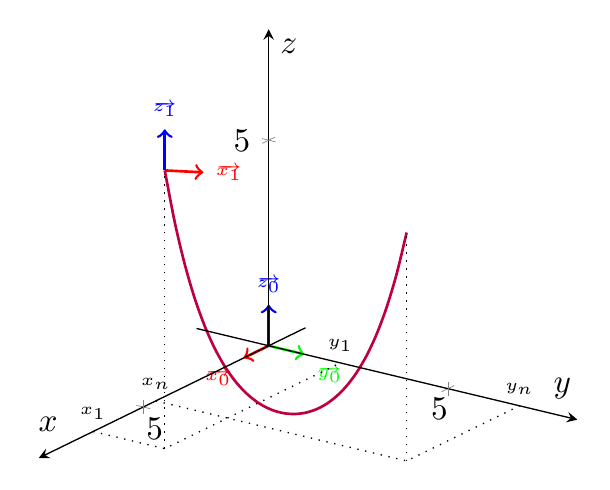
\begin{tikzpicture}[scale=1.2]
                \begin{axis}[view={125}{20},
                    axis lines=center,axis on top,
                    xlabel=$x$,ylabel=$y$,zlabel=$z$,
                    no marks,axis equal,
                    xmin=0,xmax=7,ymin=0,ymax=6,zmin=0,zmax=7,
                    enlargelimits={upper=0.1}]
    
                    % R0
                    \draw[thick,->, red] (0,0,0) -- (1,0,0) node[anchor=north east] (x0) {\tiny $\overrightarrow{x_0}$};
                    \draw[thick,->, green] (0,0,0) -- (0,1,0) node[anchor=north west] (y0) {\tiny $\overrightarrow{y_0}$};
                    \draw[thick,->, blue] (0,0,0) -- (0,0,1) node[anchor=south] (z0) {\tiny $\overrightarrow{z_0}$};
    
                    % R1
                    \draw[thick,->, red] (7,2,6.769) -- ++(-0.4,0.8,0) node[anchor=west] (x1) {\tiny $\overrightarrow{x_1}$};
                    \draw[thick,->, blue] (7,2,6.769) -- ++(0,0,1) node[anchor=south] (z1) {\tiny $\overrightarrow{z_1}$};
    
                    % Tether
                    \addplot3[
                        samples y=0,
                        smooth, thick, color=purple,
                        domain=2:7
                        ] ({8-0.5*x},{x},{cosh(x-4.6)});
                    
                    % label points
                    \node [above] at (7,0,0) {\tiny $x_1$};
                    \node [above] at (0,2,0) {\tiny $y_1$};
                    \node [above] at (4.5,0,0) {\tiny $x_n$};
                    \node [above] at (0,7,0) {\tiny $y_n$};
    
                    % Dots
                    \draw[dotted] (7,0,0) -- (7,2,0) -- (0,2,0);
                    \draw[dotted] (7,2,0) -- (7,2,6.769);
                    
                    \draw[dotted] (4.5,0,0) -- (4.5,7,0) -- (0,7,0);
                    \draw[dotted] (4.5,7,0) -- (4.5,7,5.556);
                \end{axis}
            \end{tikzpicture}
            \caption{Dans le repère du monde}
            \label{fig:3d_plot}
        \end{subfigure}
        \hfill
        \begin{subfigure}[b]{0.45\textwidth}
            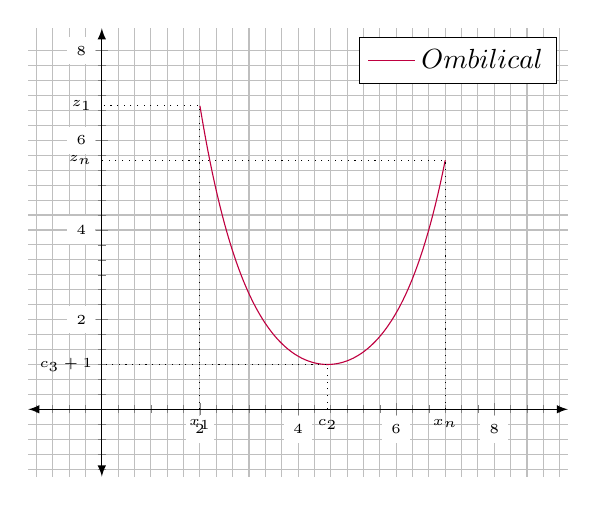
\begin{tikzpicture}
                \begin{axis}[
                        xmin=-1,   xmax=9,
                        ymin=-1,   ymax=8,
                        grid=both,
                        axis lines=middle,
                        minor tick num=5,
                        enlargelimits={abs=0.5},
                        axis line style={latex-latex},
                        ticklabel style={font=\tiny,fill=white},
                        xlabel style={at={(ticklabel* cs:1)},anchor=north west},
                        ylabel style={at={(ticklabel* cs:1)},anchor=south west}
                    ]
                    \addplot [
                        domain=2:7, 
                        samples=100, 
                        color=purple,
                        ]
                        {cosh(\x - 4.6)};
                    \addlegendentry{$Ombilical$}

                    % Labels
                    \node[below] at (2,0) {\tiny $x_1$};
                    \node[below] at (7,0) {\tiny $x_n$};
                    \node[left] at (0,6.769) {\tiny $z_1$};
                    \node[left] at (0,5.556) {\tiny $z_n$};
                    \node[left] at (0,1) {\tiny $c_3 + 1$};
                    \node[below] at (4.6, 0) {\tiny $c_2$};

                    % Dots
                    \draw[dotted] (2,0) -- (2,6.769) -- (0,6.769);
                    \draw[dotted] (4.6,0) -- (4.6,1) -- (0,1);
                    \draw[dotted] (7,0) -- (7,5.556) -- (0,5.556);
                \end{axis}
            \end{tikzpicture}
            \caption{Dans le repère de l'ombilical}
            \label{fig:2d_plot}
        \end{subfigure}
        \caption{Modélisation de l'ombilical en 3 dimensions}
    \end{figure}
    
    Pour résoudre ce système, on utilise un solveur numérique. Lors de l'implémentation en \gls{Cpp} de cette étape d'initialisation, la librairie \gls{GSL}\footnote{\url{https://www.gnu.org/software/gsl/}} a été utilisée. Une fois les paramètres déterminés, on est en mesure de déterminer la position initiale de chaque n\oe ud dans le repère de l'ombilical, puis dans le repère du monde.

\subsection{Implémentation}
    L'implémentation d'un \gls{Plugin} \gls{Gazebo} permet de simuler le comportement de l'ombilical dans l'environnement de simulation. Ce \gls{Plugin} est basé sur l'instanciation d'objets de type \textit{Tether} et \textit{TetherElement}. L'objet \textit{Tether} possède les paramètres de simulation de l'ombilical, tandis que l'objet \textit{TetherElement} représente un tronçon de cet ombilical. Un diagramme de classe est présenté en \textsc{Figure}~\ref{fig:uml_class} et montre les différents attributs et méthodes associées à chaque classe.
    
    La \textit{Tether} utilise une structure de liste doublement chaînée\footnote{structure de données liée qui consiste en un ensemble n\oe uds liés les uns aux autres par des références au n\oe uds voisins.} de \textit{TetherElement}. Chaque \textit{TetherElement} possède alors une référence vers l'élément le précédant et l'élément le suivant, comme le montre la \textsc{Figure}~\label{fig:goubly_linked_list}. La \textit{Tether} ne possède ainsi qu'une référence vers le premier et le dernier n\oe ud de la chaîne, nommés respectivements \textit{head} et \textit{tail}. Il est ensuite possible de parcourir la chaîne de \textit{TetherElement} dans les deux sens en utilisant les références gardées par les \textit{TetherElement} eux-mêmes. 

    \begin{figure}[!htb]
        \centering
        \resizebox{0.90\textwidth}{!}{
            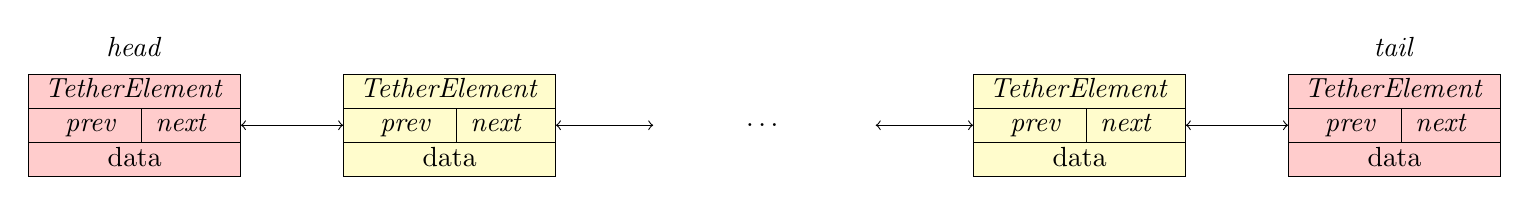
\begin{tikzpicture}
                \tikzset{TE/.style={draw, inner sep=0, outer sep=0, fill=yellow!20}}

                \node[TE, fill=red!20] (TE0) at (0,0) {\begin{tabular}{c} \textit{TetherElement} \\ \hline \hfill \textit{prev} \hfill \vline \hfill \textit{next} \hfill \\ \hline data \end{tabular}};

                \node[TE, fill=red!20] (TE4) at (16,0) {\begin{tabular}{c} \textit{TetherElement} \\ \hline \hfill \textit{prev} \hfill \vline \hfill \textit{next} \hfill \\ \hline data \end{tabular}};

                \foreach \i in {1,3} {
                    \node[TE] (TE\i) at (4*\i,0) {\begin{tabular}{c} \textit{TetherElement} \\ \hline \hfill \textit{prev} \hfill \vline \hfill \textit{next} \hfill \\ \hline data \end{tabular}};
                }
                \node[minimum width=80] (TE2) at (8,0) {\dots};
                \foreach \i in {0,1,2,3} {
                    \pgfmathtruncatemacro{\next}{\i +1}
                    \draw[<->] (TE\i) -- (TE\next);
                }

                \node (head) at (0,1) {\textit{head}};
                \node (tail) at (16,1) {\textit{tail}};
            \end{tikzpicture}
        }
        \caption{Liste doublement chainée}
        \label{fig:doubly_linked_list}
    \end{figure}

    \begin{figure}[!htb]
        \centering
        \resizebox{0.50\textwidth}{!}{
            \begin{tikzpicture}
                \begin{class}[text width=6cm]{Tether}{0,0}
                    \attribute{+ element\_mass : double}
                    \attribute{+ element\_volume : double}
                    \attribute{+ element\_length : double}
                    \attribute{+ position\_first : numpy.ndarray}
                    \attribute{+ position\_last : numpy.ndarray}
                    \attribute{+ elements : list of \textit{TetherElement}}
                \end{class}
            
                \begin{class}[text width=6cm]{TetherElement}{8.5,0}
                    \attribute{+ mass : double}
                    \attribute{+ volume : double}
                    \attribute{+ length : double}
                    \attribute{+ position : numpy.ndarray}
                    \attribute{+ velocity : numpy.ndarray}
                    \attribute{+ acceleration : numpy.ndarray}
                    \attribute{+ previous : TetherElement}
                    \attribute{+ next : TetherElement}
                    \attribute{+ K\_p : double}
                    \attribute{+ K\_d : double}
                    \attribute{+ K\_i : double}
                    \operation{+ F\_p(self) : numpy.ndarray}
                    \operation{+ F\_b(self) : numpy.ndarray}
                    \operation{+ F\_f(self) : numpy.ndarray}
                    \operation{+ Ft\_prev(self) : numpy.ndarray}
                    \operation{+ Ft\_next(self) : numpy.ndarray}
                \end{class}
            
                \aggregation{Tether}{}{~~~n}{TetherElement}
            \end{tikzpicture}
        }
        \caption{Diagramme de classe UML des classes \textit{Tether} et \textit{TetherElement}}
        \label{fig:uml_class}
    \end{figure}

\subsection{Suivi d'angles normalisés}
    Un problème avec la représentation numérique de l'orientation des solides est qu'elle est souvent normalisée, et les valeurs sont ainsi ramenées dans l'intervalle $[-\pi; \pi]$. On ne peut donc pas avoir l'orientation absolue, c'est à dire l'orientation d'un solide en prenant en compte les eventuels tours qu'il aurait pu faire sur lui-même.

    Pour résoudre ce problème, l'\textsc{Algorithme}~\ref{algo:suivi_angle} de suivi d'angles normalisés a été implémenté. Il prends en paramètres l'angle normalisé ainsi que l'angle précédemment calculé, et il retourne la valeur de l'angle absolu. L'idée de fournir l'angle précédent est de pouvoir retourner le nouvel angle qui se trouve dans le même quadrant et aussi de pouvoir suivre les sauts d'angles. Ainsi on peut suivre l'orientation absolue de solides en rotation dans l'espace, en ne fournissant que des orientations relatives ramenées dans l'intervalle $[-\pi; \pi]$, et en gardant en mémoire la précédente orientation calculée.
    
    \begin{algorithm}[!htb]
        \SetKwInOut{Input}{Entrées}
        \SetKwInOut{Output}{Sorties}
        \Entree{$angle\_normalise$, $angle\_absolu$}
        \Sortie{$angle\_absolu$}
        \Deb{
            $offset \leftarrow (angle\_absolu - angle\_normalise + \pi ) \pmod{2\pi}$ \\
            $angle\_absolu \leftarrow angle\_normalise + 2\pi \cdot offset$ \\
        }
        \Retour{$angle\_absolu$}

        \caption{Suivi d'angle} 
        \label{algo:suivi_angle}
    \end{algorithm}

    La \textsc{Figure}~\ref{fig:suivi_angle} présente les résultats de l'\textsc{Algorithme}~\ref{algo:suivi_angle} avec une angle variant dans l'intervalle $[-3\pi; 3\pi]$. On voit sur la première sous-figure l'angle réel et l'angle ramené dans l'intervalle $[-\pi; \pi]$ avec la présence de saut d'angles. Avec cette méthode, on est capable de suivre l'évolution de l'angle et de supprimer cess sauts afin de retrouver l'angle absolu visible dans la deuxième sous-figure et calculé uniquement à partir de la connaissance de l'angle normalisé.

    \begin{figure}[!htb]
        \centering
        \includegraphics[width=0.5\textwidth]{suivi_angle.png}
        \caption{Suivi d'angle}
        \label{fig:suivi_angle}
    \end{figure}


\subsection{Resultats}